%=========================================================================
% (c) 2011, 2012 Josef Lusticky <xlusti00@stud.fit.vutbr.cz>

\chapter{NTP client in Contiki OS}
For implementation of reasonably useful NTP client,
operating system must be able to set, get
and eventually adjust time.
Though not mandatory, adjusting time is important function,
if the time shall be always a monotonically increasing function.
Apart from that, communicating abilities over UDP are also required.

Thanks to uIP, described in section~\ref{sec:contiki-uip}, communication is
not a matter for Contiki OS.
Contiki is also able to use Domain Name System for IPv4 address resolution.
DNS resolution of IPv6 addresses was not implemented in Contiki OS
at the time of writing~\cite{contiki-docs}.
The main problem of NTP client implementation for Contiki is therefore total
lack of real-time support.
Not only no common interface availability, but also
almost no platform-specific code has been implemented towards time support yet.
Contiki provides basic clock interface particularly for use of timers though.
This interface is common for all supported platforms,
but the particular implementation is platform specific.

Another deal might be possible packet loss if communication uses UDP on transport layer.
The reason why this can happen often is explained in section~\ref{sec:contiki-uip}.
However, packet loss is not a matter for NTP if using either broadcast or unicast mode.
In broadcast mode, lost server packet causes no setting or adjusting time of client's
local clock.
The client simply waits without disruption for next NTP broadcast message.
If client needs to figure out it's local clock offset at the moment,
it can simply query a server using NTP unicast mode.

In unicast mode packet loss might occur either for client's query to server
or for server's response to client.
If client's query loss occurs, no server response will be sent.
Similarly, if server's response loss occurs, no message will be received by the client.
It is therefore important not to block whole system till response arrives.
%TO COMMUNICATION: In Contiki the application is invoked in response to certain events
%... This can be effectively solved by NTP Poll Interval.

For developing and testing Contiki NTP client,
the AVR Raven platform with ATmega1284P CPU~\cite{avr-datasheet} was used.
% do not mention, appendix?
How to get a working setup with Contiki on this platform is described in
%!%% CHECK THIS %%%
docs/setup.pdf file on the CD enclosed to this thesis.
%%% CHECK THIS %%%

%=========================================================================
% (c) 2011, 2012 Josef Lusticky

\section{Hardware clock interface}
Contiki features a basic clock interface with a simple goal - measuring time.
This interface provides needed calls for timers and its definition is to be found in {\it{/core/sys/clock.h}} file.
Specific implementations of this common interface are located in {\it{/cpu}} directory of Contiki source code.
The interface provides call for initialising CPU's clock system {\it{clock\_init}} that is automatically called during
boot sequence of Contiki.
The goal of the {\it{clock\_init}} call is to set up
appropriate counter registers and interrupt service routines. %! TODO .. as described in chapter..
For AVR CPU this call is implemented as C macro, which evaluates to specific setup code for each
different type of AVR CPU during compilation, and is defined in {\it{cpu/avr/dev/clock-avr.h}} file.
The setup code is not common to all CPUs because of differences among them - e.g. there are usually
only three Timer/Counter modules, but AVR ATmega1284P has four Timer/Counter modules~\cite{avr-datasheet}.

On AVR Raven, 8 bit Timer/Counter~2 clocked from 32~768~Hz watch crystal
is used by Contiki clock interface,
which is in turn used by dependent timers - refer to section~\ref{sec:contiki-timers} for details.
This 32~768~Hz watch crystal is independent of the I/O clock, can be only used
with Timer/Counter~2 and it
enables use of Timer/Counter2 as a Real Time Counter~\ref{avr-datasheet}.
%Unlike I/O clock used for clocking other Timers/Counters,
%this asynchronous crystal is also active in power-save mode~\ref{avr-datasheet}.
If Timer/Counter2 is enabled, it will keep running during sleep. The device can wake up from
either Timer Overflow or Output Compare event from Timer/Counter2 if the corresponding
Timer/Counter2 interrupt enable bits are set in TIMSK2, and the Global Interrupt Enable bit in
SREG is set.
If Timer/Counter2 is not running, Power-down mode is recommended instead of Power-save
mode.
The Timer/Counter2 can be clocked both synchronously and asynchronously in Power-save
mode. If the Timer/Counter2 is not using the asynchronous clock, the Timer/Counter Oscillator is
stopped during sleep. If the Timer/Counter2 is not using the synchronous clock, the clock source
is stopped during sleep. Note that even if the synchronous clock is running in Power-save, this
clock is only available for the Timer/Counter2.


Timer/Counter~2 is used in Clear Timer on Compare Match (CTC) mode by Contiki.
In this mode the counter register (TCNT2) is cleared to zero when the counter
value matches the value in output compare register (OCR2A).
The OCR2A register defines the top value for the counter, hence also its resolution.

% PRESCALER
For Timer/Counter2, the possible prescaled selections are: clk T2S /8, clk T2S /32, clk T2S /64,
clkT2S/128, clkT2S/256, and clkT2S/1024. Additionally, clkT2S as well as 0 (stop) may be selected.

% write to OCR2A
If the interrupt is enabled, the interrupt handler routine can be used for updating
the TOP value. However, changing TOP to a value close to BOTTOM when the counter is run-
ning with none or a low prescaler value must be done with care since the CTC mode does not
have the double buffering feature. If the new value written to OCR2A is lower than the current
value of TCNT2, the counter will miss the compare match.

CTC

$f = $

%At least one of those is always 16 bit wide
%This extra module on AVR ATmega1284P is used for
% three vs. 3

%clock\_seconds
%CLOCK\_SECOND
This is however enough for implementing a reasonable time interface and using it for NTP client later.

% ntp interface extending the clock library, similar to posix calls

%!!AVR

Adjusting time - COMPARE\_REGISTER = 31 => 128Hz => 1s = 1s
FREQ = 32768/8 / 32
COMPARE\_REGISTER = 30 => ca132.129Hz => 1s = ca1.032258s
FREQ = 32768/8 / 31
COMPARE\_REGISTER = 32 => 124.12per => 1s = 0.96p
FREQ = 32768/8 / 33

=> fastest adjust is 0,03s / s


Each TCNT2 increment is $\frac{1}{128 \times 32} \doteq 0,000244$ s
2,44ms minimum clock slew
This is also minimal possible clock adjustment.


Adjustments will influence the timers.
Applications requiring uninfluenced timers
are therefore advised to use rtimers, described in section~\ref{sec:contiki-timers},
because they use separate hardware clock
unaffected by NTP client.


%=========================================================================
% (c) 2011, 2012 Josef Lusticky

\section{Operating system time interface - TODO}
%Since there is no way of setting, getting and adjusting the time in Contiki OS,
%the interface for setting, getting and adjusting time was developed in this thesis.
New structure for expressing time values was implemented.
This structure is similar to POSIX {\it{timespec}} structure,
described in section~\ref{sec:others-posix}.
However, name was chosen {\it{time\_spec}} to avoid collision with
existing POSIX-compliant systems.
\begin{lstlisting}
struct time_spec {
  long sec;
  long nsec;
};
\end{lstlisting}
This structure consists of two signed long values for expressing seconds and nanoseconds.
The value 0 seconds and 0 nanoseconds is equal to Unix prime epoch (1st January 1970).
In case of seconds part, the 32-bit signed long value was chosen because
it can conveniently
represent real-time values as well as local clock adjustment values, which may also be negative.
%! The existing value {\it{seconds}}, representing uptime in Contiki, is of the unsigned long type.
Such time representation will wrap around in year 2038 and is facing
what is commonly known as the year 2038 problem~\cite{posix}.

In case of nanoseconds part, the 32-bit signed long value was chosen because
one second has 1~000~000~000 nanoseconds and it is
desirable to be able to express positive as well as negative values for local clock adjustments.
As 32-bit signed long type shall be able to express values from -$2^{31}$-1 (-2~147~483~647)
to $2^{31}$-1 (2~147~483~647)~\cite{c99},
such representation will therefore never wrap around.

It should be noted that signed long data type does not have to always result in a 32-bit variable -
it is up to compiler what data width it chooses for each data type.
But as ISO C99 standard states, the maximum value for an object of type signed long
shall be greater or equal $2^{31}$-1 (2~147~483~647)~\cite{c99}.
This in fact results in at least 32-bit variable unless the compilation setting is changed.
Next to this, as the already presented variable {\it{seconds}} is of unsigned long type,
the value {\it{sec}} in {\it{time\_spec}} structure %and {\it{boottime}}
shall be of the same data width as arithmetic operations are made on them.

Usage of unsigned data type delays the wrap around problem to year 2106,
however will disable use of negative values needed for adjusting local clock.
%As current NTP Era ends 2036 code has to be changed anyway...~\cite{ntp-y2k}.

Setting the current time is only possible within one second precision -
finer time setting must be made through time adjustments described further.
Implemented {\it{clock\_set\_time}} function computes when the system started
in seconds since the Epoch and saves the result in newly implemented {\it{boottime}} variable.

Not only no variables incremented every interrupt nor any internal clock registers
are affected, but also already presented variable {\it{seconds}} is not modified.
This variable, counting uptime in seconds,
is particularly used by stimers in Contiki
and modifying it would lead to misbehaviour of stimer library
described in section~\ref{sec:contiki-timers}.

Thanks to this newly implemented {\it{clock\_set\_time}} function and {\it{boottime}} variable,
running Contiki system is able to tell uptime, current time and
time when was the system booted.
\begin{lstlisting}
volatile unsigned long boottime;

void
clock_set_time(unsigned long sec)
{
  boottime = sec - seconds;
}
\end{lstlisting}

Getting the correct current time is only possible if it was set using
the {\it{clock\_set\_time}} function before.
Newly implemented function {\it{clock\_get\_time}} is then able to tell the
current time in seconds since the Epoch by simply adding {\it{boottime}},
and {\it{seconds}}.
%! TODO
Nanoseconds part is filled using {\it{scount}} variable counting number of
interrupts within a second.
Since this variable is incremented every interrupt and there are {\it{CLOCK\_SECOND}} interrupts
per second, it is possible to get resolution of $\frac{1~000~000~000}{CLOCK\_SECOND}$ ns.
The same resolution have Contiki timers, described in section~\ref{sec:contiki-timers}.
\begin{lstlisting}
void
clock_get_time(struct time_spec *ts)
{
  ts->sec = boottime + seconds;
  ts->nsec = (1000000000 / CLOCK_SECOND) * scount;
}
\end{lstlisting}
Because {\it{1000000000}} and {\it{CLOCK\_SECOND}} are both constants, the compiler is able to
calculate the result of division during compile time.
Furthermore as both numbers are integers, the result is integer as well~\cite{c99}.
The most of CPU time is therefore spent on multiplication.
E.g. if the code is compiled using GCC version 4.3.5,
multiplication of two 32-bit variables takes 33 instructions including {\it{call}} and {\it{ret}}
instructions for entering and returning from the {\it{\_\_mulsi3}} routine, which computes
the result of multiplication.
%avr-objdump
According to AVR Instruction Set manual~\cite{avr-instruction-set},
this results in 48 clock cycles overhead,
which takes 3~000 nanoseconds assuming 16MHz CPU clock.
The timestamp provided is therefore not exact.
However, since this consumed time strongly depends on architecture and compiler specifications,
no correction was implemented to remove this inaccuracy.
The application must be instead aware that the timestamp is not exactly accurate.

TODO: Greater precision is further implemented by reading counter register.

TODO: Adjust time
POSIX:
Time values that are between two consecutive non-negative integer multiples
of the resolution of the specified clock are truncated down to the smaller multiple of the resolution.


%=========================================================================
% (c) 2011, 2012 Josef Lusticky

\section{NTP client code}
The client itself is implemented as a Contiki process.
Parameters such as remote port, local port or poll interval
can be configured using standard C define macro.
The client can communicate using both,
the NTP broadcast mode and the NTP unicast mode.
The unicast mode can be turned off by specifying no remote host.

Structure representing NTP message was borrowed from OpenNTPD daemon
and Dragonfly NTP daemon.
This structure is not using the GCC extension for representing a bit field,
instead uses a single 8-bit integer called {\it{status}}
for Leap Indicator, Version Number and Mode fields of NTP packet
described in section~\ref{sec:ntp-network}.
Accessing each field of the {\it{status}} byte is done using bitmasks.
Unlike using the bit field extension,
such a design is compliant with the standard C language.


%Even if {\it{tmpts.sec}} value is greater than {\it{ts.sec}} value,
%subtracting and casting to signed type gives correct (negative) result~\cite{c99}.
%Assuming 32-bit data types this will work until 2038 when wrap around can occur due to difference
%between {\it{ts.sec}} and {\it{tmpts.sec}} greater than $2^{31}$-1 (2~147~483~647).
%But as NTP Era 0 ends 2036 the NTP client code must be changed in the future anyway~\cite{ntp-y2k}.

%! TODO

%Adjusting time
%1/128/32 = 0.000244141
%0.000244141x32x127+0.000244141x31 == smallest possible adjustment == 244us

%% SENDING NTP TIMESTAMP
The transmit timestamp sent by the client can be set to any arbitrary value.
This is in compliance with the NTPv4 specification~\cite{rfc5905}.
It is however important for the client to store the sent timestamp,
since it is later used by the client to check the server's response.
Contiki NTP Client fills and checks only the seconds part of NTP timestamp,
because the timestamp should be as accurate as possible and the
conversion from nanoseconds to NTP fraction part would increase the interval
between determination of the timestamp and dispatch of the packet.

After the filled NTP packet is sent, the client schedules
sending of a next NTP packet in $2^{\tau}$ seconds
using the event timer library.
In NTPv4, $\tau$ ranges from 4, resulting in poll interval 16 seconds,
to 17, resulting in poll interval 36 hours.
However, the event timer library imposes a limit to scheduled time.
This limit is platform specific and depends on {\it{CLOCK\_SECOND}} value.
The $\tau$ value can not be greater than 8 on AVR Raven assuming 128 interrupts per second.
Upon scheduling the event timer, the client process yields
and another process can be run.
The client process is later invoked either by the uIP stack event
announcing the server response
or by the event timer in case no server response arrived.
Event timer is therefore effectively
dealing with possible packet loss described in section~\ref{sec:design-network}.

When the server response arrives,
determinating the destination timestamp is one of the first thing the client does.
After that, the client makes packet sanity tests including
checking whether the response is from synchronised server.

A determination of the NTP communication mode follows.
In unicast mode, the seconds field of Originate timestamp
is compared with the stored sent timestamp.
The received packet is considered bogus in case of mismatch and further processing is stopped.
Otherwise are the NTP timestamps converted to local timestamp format and
the local clock offset computed as described in section~\ref{sec:ntp-algorithms}.
After the local clock offset is computed,
the stored transmitted timestamp is immediately set to zero
to protect against replay of the last transmitted packet.

In broadcast mode, the received packet is always considered correct
and the local clock offset is computed as the difference between the local stored timestamp
and the transmit timestamp received.
As one could expect, the local clock offset determined from the broadcast mode
is less accurate then from the unicast mode.

Due to a different origin of the Unix and NTP epoch,
number of seconds between NTP and Unix epoch,
is subtracted from seconds part of NTP timestamp.
But the conversion from fraction part of long 64-bit NTP timestamp to nanoseconds,
used in the local timestamp structure,
is one of the most problematic tasks for memory constrained systems.
An accurate conversion requires either floating point operations or operations with 64 bit numbers.
The conversion is given by
$nsec = fractionl \times 10^9 \div 2^{32}$, where $nsec$ is the nanoseconds part of the local timestamp
and $fractionl$ is the fraction part of long 64-bit NTP timestamp.
Since there is no native hardware support for floating point nor for 64-bit arithmetic,
GCC would supply these operations in form of library called {\it{libgcc}},
which causes significantly bigger resulted binary file.
The greatest common divisor of $10^9$ and $2^{32}$ is $2^9$,
so in fact, a relatively simple multiplication of $fractionl$ by $\frac{5^9}{2^{23}}$ must be computed.
This can be computed using sequential divisions and multiplications,
which in turn can be done on 32 bits using shifts and additions~\cite{c99}.
\begin{lstlisting}[caption=Conversion from NTP fraction part to nanoseconds]
unsigned long
fractionl_to_nsec(uint32_t fractionl)
{
  unsigned long nsec;
  nsec = fractionl;
  nsec = (nsec >> 1) + (nsec >> 3); // nsec = nsec/2 + nsec/8 = (5*nsec)/8
  nsec = (nsec >> 1) + (nsec >> 3); // nsec = (5*nsec) / 8 = (25*fractionl)/64
  nsec = (nsec >> 1) + (nsec >> 3); // nsec = fractionl * 5^3/2^9
  /* Now we can multiply by 5^2 because then the total
   * multiplication coefficient for the original number fractionl
   * will be: fractionl * (5^5)/((2^3)^4) = fractionl * 0.762939453,
   * which is less then 1, so it can not overflow.
   */
  nsec = (nsec << 1) + nsec + (nsec >> 3); // nsec*3 + nsec/8 = (25*nsec) / 8

  nsec = (nsec >> 1) + (nsec >> 3);
  nsec = (nsec >> 1) + (nsec >> 3);

  /* Again we can multiply by 5^2.
   * Total coefficient will be fractionl * (5^9)/((2^3)^7) = fractionl * 0.931322575
   */
  nsec = (nsec << 1) + nsec + (nsec >> 3); // nsec*3 + nsec/8 = (25*nsec) / 8

  /* Last shift to agree with division by 2^23 can not be
   * done earlier since the coefficient would always be greater than 1.
   */
  nsec = nsec >> 2;
  return nsec;
}
\end{lstlisting}
As the code comments say, an extra attention must be taken of the overall
multiplication coefficient,
that can not be greater than 1 in any step.
Because $fractionl$ can be of any value between $0$ and $2^{32}-1$,
the overall coefficient greater than 1 could cause overflow and an unexpected result.

According to output from the {\it{avr-size}} tool,
when compiled with GCC 4.3.5,
using the 64-bit arithmetic for conversion
takes 656 bytes more in %program section of
resulted binary file (GCC supplies routine for multiplication and shifting 64-bit integers)
and floating point operation takes 3~358 bytes more
than the developed algorithm.

It must be noted, that the above presented conversion is not exactly accurate, particularly
because of loosing the least significant bits by the first shifts.
However, this conversion gives maximum error of 5 nanoseconds for all possible values of $fractionl$,
which is totally adequate for most platforms without floating point unit or
for platforms where usage of 64-bit arithmetic is expansive.
Beside significantly smaller memory requirements,
this algorithm gives on AVR Raven even more accurate results than the libgcc
floating point library supplied by GCC.


In the next step after conversions, the local clock offset is computed
as given in section~\ref{sec:ntp-algorithms}.
Depending on the absolute value of the local clock offset,
the system time is either set or adjusted using the {\it{clock\_set\_time}}
and {\it{clock\_adjust\_time}} call respectively.
The clock is set if the time difference is equal or greater than
treshold value, which 3 seconds by default. %!TODO
The reference NTP implementation uses 125 ms~\cite{rfc5905}
It has been the Internet
experience that the need to change the system time in increments
greater than +-128 ms is extremely rare and is usually associated
with a hardware or software malfunction or system reboot~\cite{rfc1589}.


%
% NEGATIVE result for the first time
%In some scenarios where the initial frequency offset of the client is
  %relatively large and the actual propagation time small, it is
   %possible for the delay computation to become negative.  For instance,
   %if the frequency difference is 100 ppm and the interval T4-T1 is 64
   %s, the apparent delay is -6.4 ms.  Since negative values are
   %misleading in subsequent computations, the value of delta should be
   %clamped not less than s.rho, where s.rho is the system precision
   %described in Section 11.1, expressed in seconds~\cite{rfc5905}.
%


%=========================================================================
% (c) 2011, 2012 Josef Lusticky

\section{Network communication}
The 6LoWPAN Adaptation Layer % see Interconnecting smart objects with IP
% IEEE 802.15.4
as RFC~4944 written by 6lowpan working group of IETF
made the underlaying IEEE 802.15.4 layer
look like an IPv6 link~\cite{6lowpan} and
\begin{figure}
  \centering
  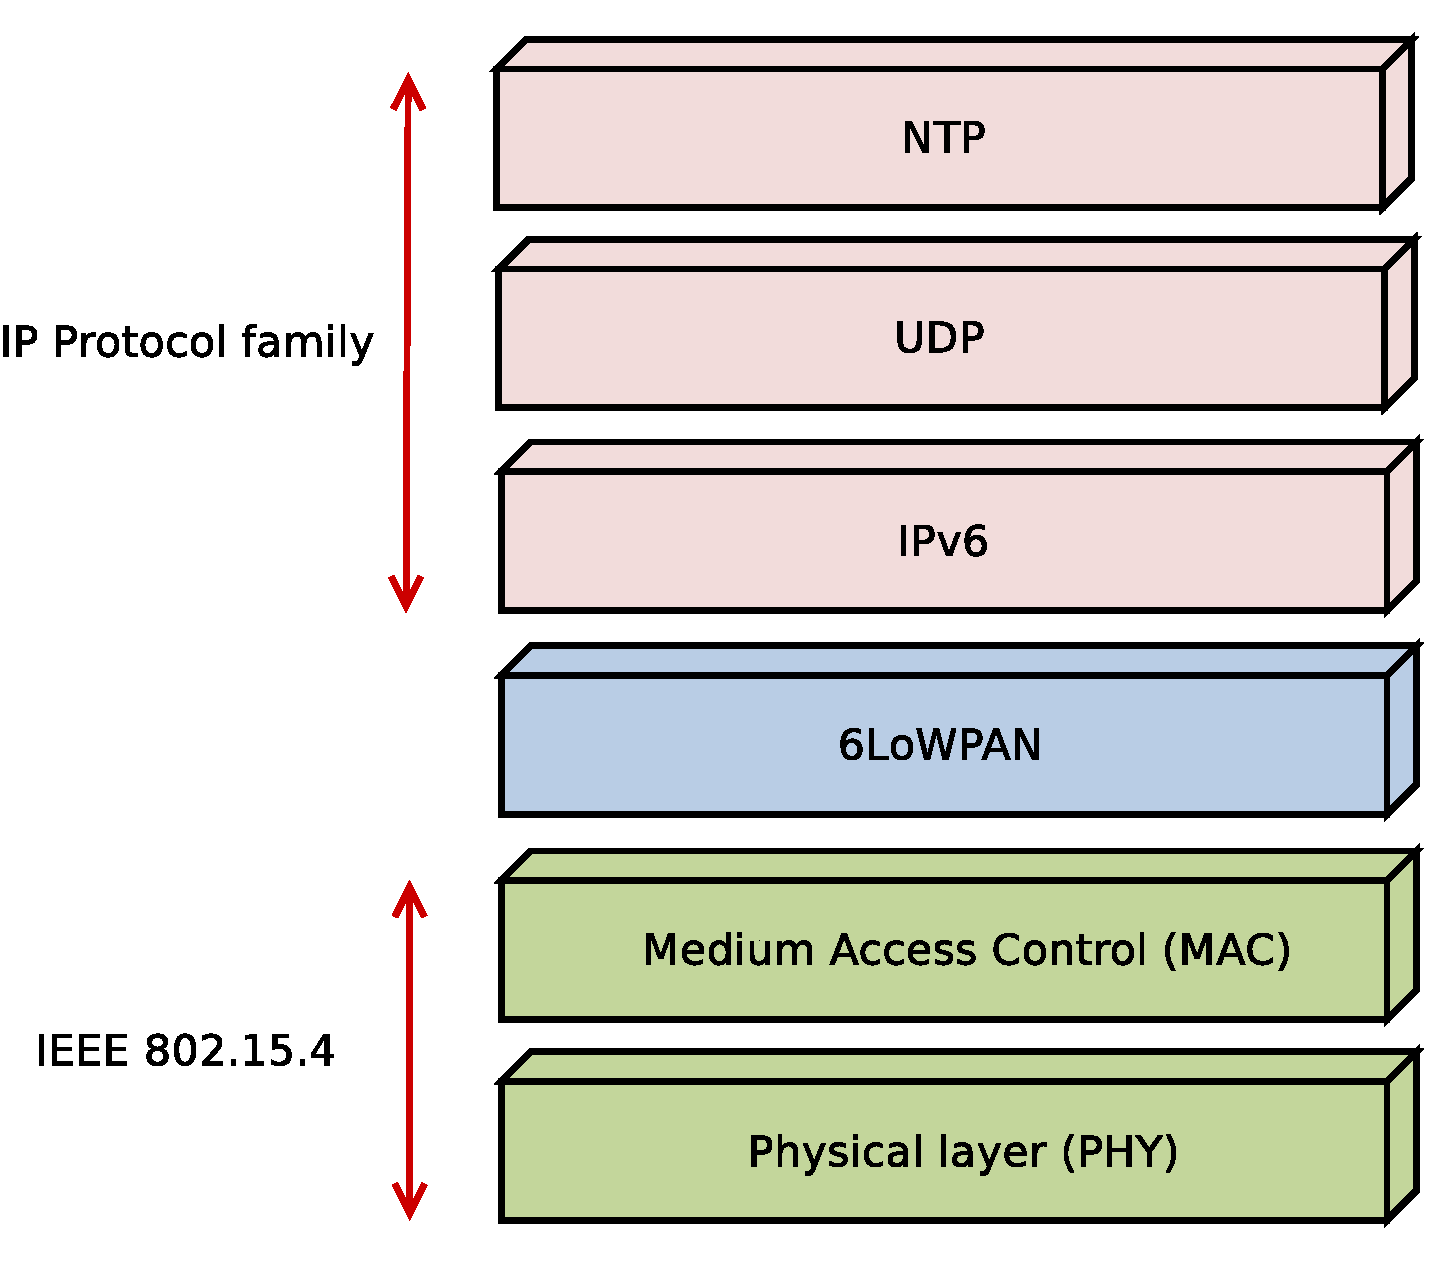
\includegraphics[width=9cm,keepaspectratio]{fig/6lowpan.pdf}
  \caption{Communication stack with 6lowpan layer}
  \label{fig:implementation-6lowpan}
  \bigskip
\end{figure}

NTP server can be specified in Makefile or
during compilate time using {\it{REMOTE\_HOST}} define.
%! TODO
TODO: If no host is specified,
NTP client assumes NTP broadcast communication mode.


% There is no IPv4 support...

%The uIP packet buffer is accessed through
%the uip\_buf array and is used to hold incoming and outgoing packets.
%The device driver should place incoming data into this buffer.
%When sending data, the device driver should read the link
%level headers and the TCP/IP headers from this buffer.
%The size of the link level headers is configured by the UIP\_LLH\_LEN
%define and in case of Ethernet it is 14.

%The application data need not be placed in this buffer, so
%the device driver must read it from the place pointed to by the
%uip\_appdata pointer %as illustrated by the following example:

Routing to Meinberg NTP primary server.
Measurements made using this setup are discussed in chapter~\ref{chap:measurements}.

